\section{Grundaufbau}
    Der Ballwerfer ist so konzipiert, das er aus einem fix stehenden Basismodul besteht, 
    welches in der Mitte des Startbereiches positioniert wird. Die Abwurfeinheit, welche 
    den Ballwurfmechanismus und die Ballzuführung beinhaltet, ist auf dem Basismodul 
    drehend gelagert. Weiter ist auch das Smartphone für die Korberkennung und alle 
    Steuereinheiten auf dem Basismodul angebracht. Das Startsignal wird mittels W-Lan 
    von einem externen Labtop übertragen.\\
    Der ganze Aufbau des Ballwurfmechanismus ist sehr simple gehalten. Er besteht 
    hauptsächlich aus zwei 5mm dicken Acrylglasplatten, in welcher alle mechanischen 
    Vorrichtungen gelagert sind. Durch diesen Aufbau können Änderungen schnell und 
    einfach angepasst werden. Die Ausrichtung des Abwurfmechanismus erfolgt durch 
    einen sehr flachen Steppermotor, welcher in der drehenden Abwurfeinheit angebracht 
    ist. Dadurch wird die Bauhöhe des Ballwerfers tief gehalten, was einen grossen 
    Stabilitätsvorteil bietet. Die Drehachse der Abwurfeinheit ist an der Spitze des 
    Ballwerfers mit einem Bolzen angebracht. Somit bleibt die Abwurfposition der 
    Tennisbälle konstant am gleichen Ort. Die Tennisbälle werden durch zwei 
    Beschleunigungsräder beschleunigt. Die Beschleunigungsräder werden je einzeln 
    über eine Übersetzung mit einem Brushlessmotor auf Touren gebracht. Die Schwungräder 
    drehen gegenläufig und die Tennisbälle werden dazwischen hindurchgeführt und 
    abgeworfen. Die Zuführung der Tennisbälle zu den Beschleunigungsräder erfolgt mit 
    einem geregelten Förderband. Das Förderband transportiert die Bälle mit einer 
    konstanter Geschwindigkeit zu den Beschleunigungsräder, damit alle Tennisbälle die 
    gleiche Startenergie aufweisen. Dadurch ist eine gleichmässige Wurfweite und eine 
    hohe Reproduzierbarkeit gewährleistet.

    \subsection{Hauptcontroller}
        Die gesamte Hardware wird über das Freedom Board\footnote{Development-Board vom 
        Hersteller Freescale, Typ FRDM-KL25Z} gesteuert. Dieses Board hat ein internen UART\footnote{\textbf{U}niversal \textbf{A}synchronous \textbf{R}eceiver 
        \textbf{T}ransmitter, eine serielle Schnittstelle} to USB Converter, über diesen 
        der Host mit dem Board kommuniziert. Die Software des Boards besteht aus einem 
        Betriebssystem, dessen Haupttask kontinuierlich den UART Eingangspuffer abruft 
        und die angekommenen Befehle ausführt. Ein wichtiger nur einmal gebrauchter Task 
        ist die Initialisierung des Stepperboards, siehe Anhang (??). Der Controller 
        verfügt über zwei SPI-Schnittstellen. Am einen ist das besagte Stepperboard und 
        an der Anderen die beiden Brushless-Boards angeschlossen. Weiter ist ein PWM-Port 
        verwendet, um den Motor der Ballnachführung anzutreiben, siehe Kapitel 
        \ref{sec:Foerderband}.        
    \subsection{Spannungsversorgung}       
        \begin{wrapfigure}{r}{0.35\textwidth}
           	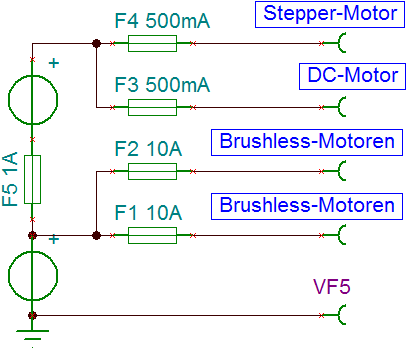
\includegraphics[width=0.35\textwidth,clip,trim=0mm 2mm 0mm 1mm]
           	{Enddokumentation/Bilder/BeschaltungNetzteile.png}
           	\centering
           	\caption{Schema der Spannungsversorgung} 
           	\label{abb:Spannungsversorgung}
        \end{wrapfigure}
        Gemäss Datenblatt sind die verwendeten Brushless-Motoren mit einer Versorgungsspannung 
        von $12\si{\volt}$ bei einem maximalen Strom von $11\si{\ampere}$ spezifiziert. 
        Der Steppermotor und der DC-Motor sind gemäss Datenblatt für eine Betriebsspannung 
        von $24\si{\volt}$ ausgelegt. Die Spannungsversorgung werden mit zwei Server-Netzteile 
        realisiert, die je $12\si{\volt}$ mit maximal $60\si{\ampere}$ liefern. Aus 
        Sicherheitsgründen wird für jeden Motor eine separate Sicherung verwendet. Das Schema 
        in Abbildung \ref{abb:Spannungsversorgung} zeigt, wie die Spannungsversorgung 
        realisiert ist. Das Freedom-Board wird über USB vom Akkumulator des Smartphone 
        gespeist. Sämtliche Datenblätter zu den verwendeten Motoren sind im Anhangsdokument 
        angefügt.